\chapter{Gravitational-Wave Cosmology}
\label{chap:dark-siren-cosmology}

\section{Standard Siren Cosmology}

The detection of \acfp{GW} from \acp{CBC} have opened a transformative avenue in modern cosmology. These events acts as \textit{standard sirens}, the gravitational analog of standard candles, as the luminosity distance ($d_L$) to a \ac{GW} source is directly encoded in the strain amplitude and frequency evolution of the \ac{GW}. The amplitude, corrected for antenna pattern and inclination, provides a direct, calibration-free distance measurement under the assumption of general relativity.

From~\citet{maggiore2007gravitational}, the strain measured by a GW detector can be expressed as:
\begin{align}
h(t) = \frac{4}{d_L} \left( \frac{G\mathcal{M}_z}{c^2} \right)^{5/3}
       \left( \pi f(t) \right)^{2/3} F(\iota, \psi, \theta, \phi)
\label{eq:gw_strain}
\end{align}
where:
\vspace{-1em}
\begin{itemize}
    \item $h(t)$ is the strain measured at time $t$,
    \vspace{-1em}
    \item $d_L$ is the luminosity distance to the source,
    \vspace{-1em}
    \item $\mathcal{M}_z = (1+z)\mathcal{M}$ is the redshifted chirp mass,
    \vspace{-1em}
    \item $f(t)$ is the instantaneous GW frequency,
    \vspace{-1em}
    \item $F(\iota, \psi, \theta, \phi)$ is a function that captures the detector response depending on inclination angle $\iota$, polarization angle $\psi$, and sky position $(\theta, \phi)$.
\end{itemize}

The amplitude scaling with $1/d_L$ makes it possible to extract the luminosity distance directly from the signal, once the source's intrinsic properties and orientation are marginalized over. Furthermore, the $1/d_L$ scaling, in comparison to the $1/d_L^2$ scaling of \ac{EM} signals, means that \ac{GW} signals allow observations of sources at much larger distances, making them ideal for cosmological applications.

The direct self-calibrated measurement of the luminosity distance from the \ac{GW} signal is a key advantage of standard sirens over traditional \ac{EM} standard candles. This is in stark contrast to traditional \ac{EM} standard candles, such as \ac{SNe}, where the distance is inferred from the observed flux and requires a calibration step to account for the intrinsic brightness of the source. The \ac{GW} signal is also less affected by the intergalactic medium, as it is not subject to scattering or absorption like \ac{EM} signals. This allows for a more direct measurement of the distance to the source not affected by dust extinction or other astrophysical uncertainties that plague \ac{EM} observations. This makes \ac{GW} standard sirens a powerful tool for cosmology.

The concept of standard sirens was first introduced by Bernard F. Schutz, who noted that if the redshift of a \ac{GW} source can be measured, one could use \ac{GW} events to trace the  expansion history of the Universe, in particular an independent measurement of the Hubble constant ($H_0$) \citep{schutz1986determining}. This is due to the relation between the luminosity distance, redshift and the Hubble constant, in a flat \(\Lambda\)CDM cosmology, being:
\begin{align}
    d_L = \frac{c(1+z)}{H_0} \int_0^z \frac{dz'}{\sqrt{(1+z')^3\Omega_m + \Omega_\Lambda}}
\end{align}

Unlike traditional \ac{EM} methods, which require cross-calibration across multiple rungs of the distance ladder (parallax, Cepheids, SNe Ia) with each step introducing uncertainties that compound, the standard siren approach provides a direct cosmological probe. This reduces systematic uncertainties and provides an independent check on other $H_0$ measurement techniques, possibly providing a solution to the Hubble tension, the current discrepancy between local and global measurements of the Hubble constant \citep{Riess:2019cxk,Planck:2018vyg}.

However, a key limitation is that while \ac{GW} detectors provide a precise measurement of $d_L$, they do not directly measure the redshift. This necessitates an independent redshift measurement to place the source on the Hubble diagram. For \textit{bright sirens}, this redshift is obtained from the host galaxy identified via an \ac{EM} counterpart. In contrast, for \textit{dark sirens}, the redshift is inferred statistically by cross-referencing the \ac{GW} localization volume with galaxy catalogs or by leveraging population-based methods, as discussed in the following sections.

This forms the basis for \textit{standard siren cosmology}, where \ac{GW} sources are used as cosmic rulers. Over the past decade, this idea has transitioned from theoretical speculation to experimental reality, primarily through observations made by the \acf{LVK} collaboration. The first \ac{GW} event, \textbf{GW150914}, was detected in 2015, marking the beginning of a new era in astrophysics and cosmology \citep{abbott2016gw150914}. Since then, the \ac{LVK} collaboration has detected numerous \ac{GW} events, including \acf{BBH} mergers, \acf{BNS} mergers, and \acf{NSBH} mergers. These observations have provided valuable insights into the nature of gravity, the formation of compact objects, and the expansion history of the Universe.

\newpage
\section{Bright vs. Dark Sirens}
Standard sirens fall into two broad categories: \textit{bright sirens} and \textit{dark sirens}, depending on whether an electromagnetic counterpart is detected.

Bright sirens are rare but powerful. A prime example is \textbf{GW170817}, a \ac{BNS} merger detected by LIGO-Virgo in 2017, which was accompanied by a short gamma-ray burst and subsequent kilonova \citep{LIGOScientific:2017adf}. This multi-messenger event enabled the unambiguous identification of its \textit{host galaxy, NGC 4993}, providing both distance (from \ac{GW}) and redshift (from optical spectroscopy) measurements. The resulting Hubble constant measurement, $H_0 = 70.0^{+12.0}_{-8.0}~\mathrm{km}~\mathrm{s}^{-1}\mathrm{Mpc}^{-1}$, was a major milestone demonstrating that \ac{GW} observations could offer an independent and competitive cosmological probe \citep{LIGOScientific:2017adf}.

Such bright sirens provide a straightforward route to cosmological inference, using independent distance and redshift measurements. However, bright sirens require specific astrophysical conditions: the emission of \ac{EM} signals strong enough to be detected, accurate sky localization, and timely follow-up by optical telescopes. Such conditions are only met for a small fraction of \ac{CBC} events, especially those involving neutron stars. Majority of the observed mergers, especially \acfp{BBH} do not produce detectable \ac{EM} counterparts, and are thus classified as dark sirens.

In the absence of a direct redshift measurement, dark sirens require a \textit{statistical approach}. This involves cross-matching the sky localization and distance posterior from the \ac{GW} event with a galaxy catalog covering the relevant region. The redshift information of a number of candidate galaxies is then used to statistically infer the likely redshift distribution of the source. This is done by constructing a \textit{\acf{LOS} redshift prior} for each \ac{GW} event, which is then used to infer the Hubble constant. The LOS redshift prior is constructed by taking into account the galaxy number density and redshift distribution within the localization volume of the \ac{GW} event. The \ac{GW} localization volume is typically much larger than the volume of a galaxy, leading to a large number of galaxies that could potentially host the \ac{GW} event. This results in a large number of potential redshift measurements, which can be used to construct a more accurate \ac{LOS} redshift prior.

The statistical nature of dark sirens allows for the inclusion of a larger number of events, as it does not rely on the detection of an \ac{EM} counterpart. This is particularly important for \ac{BBH} events, which are more common and have a higher detection rate than \ac{BNS} events. 
%The \ac{LVK} collaboration has detected a large number of \ac{BBH} events, many of which are dark sirens. 
The \acf{LVK} collaboration has detected numerous dark siren events, which have been used to constrain the Hubble constant and test cosmological models~\citep{abbott2023constraints}.

As the number of \ac{BBH} detections increases with each observing run, dark sirens will dominate the future of standard siren cosmology. However, this statistical method introduces new complexities and depends heavily on the quality and completeness of the galaxy catalog used, which plays a pivotal role in the reliability of the inferred Hubble constant. The incompleteness of the galaxy catalog can lead to biases in the inferred redshift distribution, which can affect the accuracy of the Hubble constant measurement. This is particularly important for dark sirens, as they rely on the statistical association of \ac{GW} events with galaxies in the catalog. State of the art dark siren methods have been developed to mitigate these issues, but they still rely on the quality and completeness of the galaxy catalog used. The next section discusses the current state of the art in dark siren cosmology, including the challenges and limitations of existing methods.

\section{State of the Art Dark Siren Methods}
The statistical framework for dark siren cosmology has evolved rapidly. Early implementations relied on basic overlap between GW localization volumes and precompiled galaxy catalogs. The first generation of tools, including \texttt{gwcosmo}~\citep{gray2020cosmological, gray2022pixelated, gray2023joint} and \texttt{icarogw}~\citep{mastrogiovanni2021importance, mastrogiovanni2024icarogw}, introduced a more rigorous Bayesian framework: for each \ac{GW} event, a \textit{\ac{LOS} redshift prior} is constructed using galaxy number counts and redshifts, weighted by host probability, typically modeled using stellar mass proxies such as $K$-band luminosity.

One major challenge in this process is that current galaxy catalogs, such as \texttt{GLADE+} \citep{dalya2022glade+}, are incomplete beyond low redshift (typically $ z > 0.2 - 0.3$). This incompleteness leads to a nontrivial \textit{out-of-catalog} term in the redshift prior, which must be modeled analytically using a \textit{Schechter luminosity function}~\citep{gray2023joint, chen2024testing}. This function estimates the number density of missing faint galaxies, often assuming fixed parameters (e.g., $M_*,\alpha$) calibrated from deep surveys. If this modeling is inaccurate, the resulting posterior for $H_0$ can be biased or artificially broadened.

Despite these challenges, dark siren methods have been successfully applied to increasingly large datasets. The \ac{LVK} collaboration has published joint analyses using \ac{CBC} events from the \textbf{O1, O2,} and \textbf{O3} observing runs. For instance,~\citet{abbott2021gravitational, abbott2023constraints} presented cumulative constraints on $H_0$ using numerous \ac{CBC} events, demonstrating convergence toward a 10--15\% precision regime, albeit still limited by catalog systematics.

These analyses highlight the potential of dark sirens to provide competitive cosmological constraints, especially as galaxy catalogs improve and detection rates increase. Future observing runs, such as \textbf{O4} and \textbf{O5}, are expected to significantly enhance the statistical power of dark siren cosmology, potentially reducing uncertainties in $H_0$, providing better constraints on cosmological model, and testing the validity of general relativity on cosmological scales. The next generation of \ac{GW} detectors, such as the ground-based \textbf{Einstein Telescope}~\citep{Abac:ET} and \textbf{Cosmic Explorer}~\citep{Evans:CE}, and the space-based \textbf{LISA} observatory~\citep{LISA:2024hlh}, will further enhance the sensitivity and detection rates of \ac{GW} events, opening up new avenues for cosmological exploration.

\subsection{Redshift Inference Methods}
In dark siren cosmology, two principal strategies exist for inferring the redshift of gravitational-wave sources: the \textit{catalog-based method}~\citep{gray2020cosmological,gray2023joint,chen2024testing} and the \textit{population-based method}~\citep{ezquiaga2022spectral}. The catalog method, briefly discussed earlier, statistically associates \ac{GW} sources with galaxies from a survey by constructing a redshift prior along each line of sight, derived from galaxy positions and redshifts within the \ac{GW} localization volume. This approach captures the clustering of galaxies and allows for redshift inference when direct \ac{EM} counterparts are absent, but suffers from incompleteness at higher redshifts and spatial variation in survey depth~\citep{gray2020cosmological,gray2023joint,chen2024testing}. Conversely, the population method, often referred to as the \textit{spectral siren approach}, leverages features in the observed distribution of source-frame binary parameters, especially masses, which are redshifted in the detector frame. If the intrinsic mass distribution contains recognizable structure (e.g., a cutoff or peak), its displacement due to cosmic redshift can break the mass-redshift degeneracy, enabling cosmological inference independent of galaxy surveys~\citep{ezquiaga2022spectral}. However, this approach is sensitive to modeling assumptions about the underlying binary population. 

%If the intrinsic mass distribution contains recognizable structure (e.g., a cutoff or peak), its displacement due to cosmic redshift can break the mass-redshift degeneracy, enabling cosmological inference independent of galaxy surveys. In \ac{GW} observations, the detector-frame mass is related to the source-frame mass via $m_{\text{det}} = (1 + z)\, m_{\text{source}}$, making it difficult to disentangle intrinsic masses from redshift effects without external information~\citep{ezquiaga2022spectral, gray2023joint}. However, this approach is sensitive to modeling assumptions about the underlying binary population.
Recent work has sought to improve robustness by combining dark siren methods with \textit{spectral sirens}, extracting redshift information from the observed mass distribution of \ac{GW} sources under population synthesis assumptions~\citep{ezquiaga2022spectral}. These hybrid approaches aim to reduce dependence on incomplete catalogs and mitigate selection biases while extracting maximal cosmological information from current GW detections. Recently, both \texttt{gwcosmo} and \texttt{icarogw} have been updated to support such joint inference schemes~\citep{gray2023joint, mastrogiovanni2024icarogw}.

%Although powerful and refined, these methods are still limited by the incompleteness of the currently available galaxy catalog. This thesis aims to tackle this incompleteness problem, by refining the construction of the redshift prior. This is done by \textit{restricting the galaxy catalog to its brightest subset}, effectively making the catalog more complete. The rationale being that bright galaxies are better cataloged and more reliably associated with massive halos, which are more likely to host detectable GW events. By selectively using only the top $XX\%$ of galaxies by $K$-band luminosity, one can reduce the \textit{out-of-catalog contribution}, thereby increasing precision without strongly biasing the result. The upcoming chapters describe and validate this approach using real and mock data.

\subsection{Galaxy Weighting Choices}
In the construction of the \ac{LOS} redshift prior, each host galaxy is weighted by its probability of hosting a \ac{GW} event. This probability is typically modeled as a function of the galaxy's luminosity, and relies on the assumption that the merger host probability of a galaxy is related to its luminosity in a specific band. The choice of band remains uncertain, with different bands correlating with different aspects. The blue band, for instance, correlates with star formation rate and is therefore appropriate for mergers with short time delays (coalescence shortly after formation), while the near-infrared band correlates with the total luminous mass and is thus appropriate for mergers with longer time delays (mergers in older, more evolved galaxies). It is not known how exactly galaxy color is correlated with the merger rate.

\begin{figure}[ht]
    \centering
    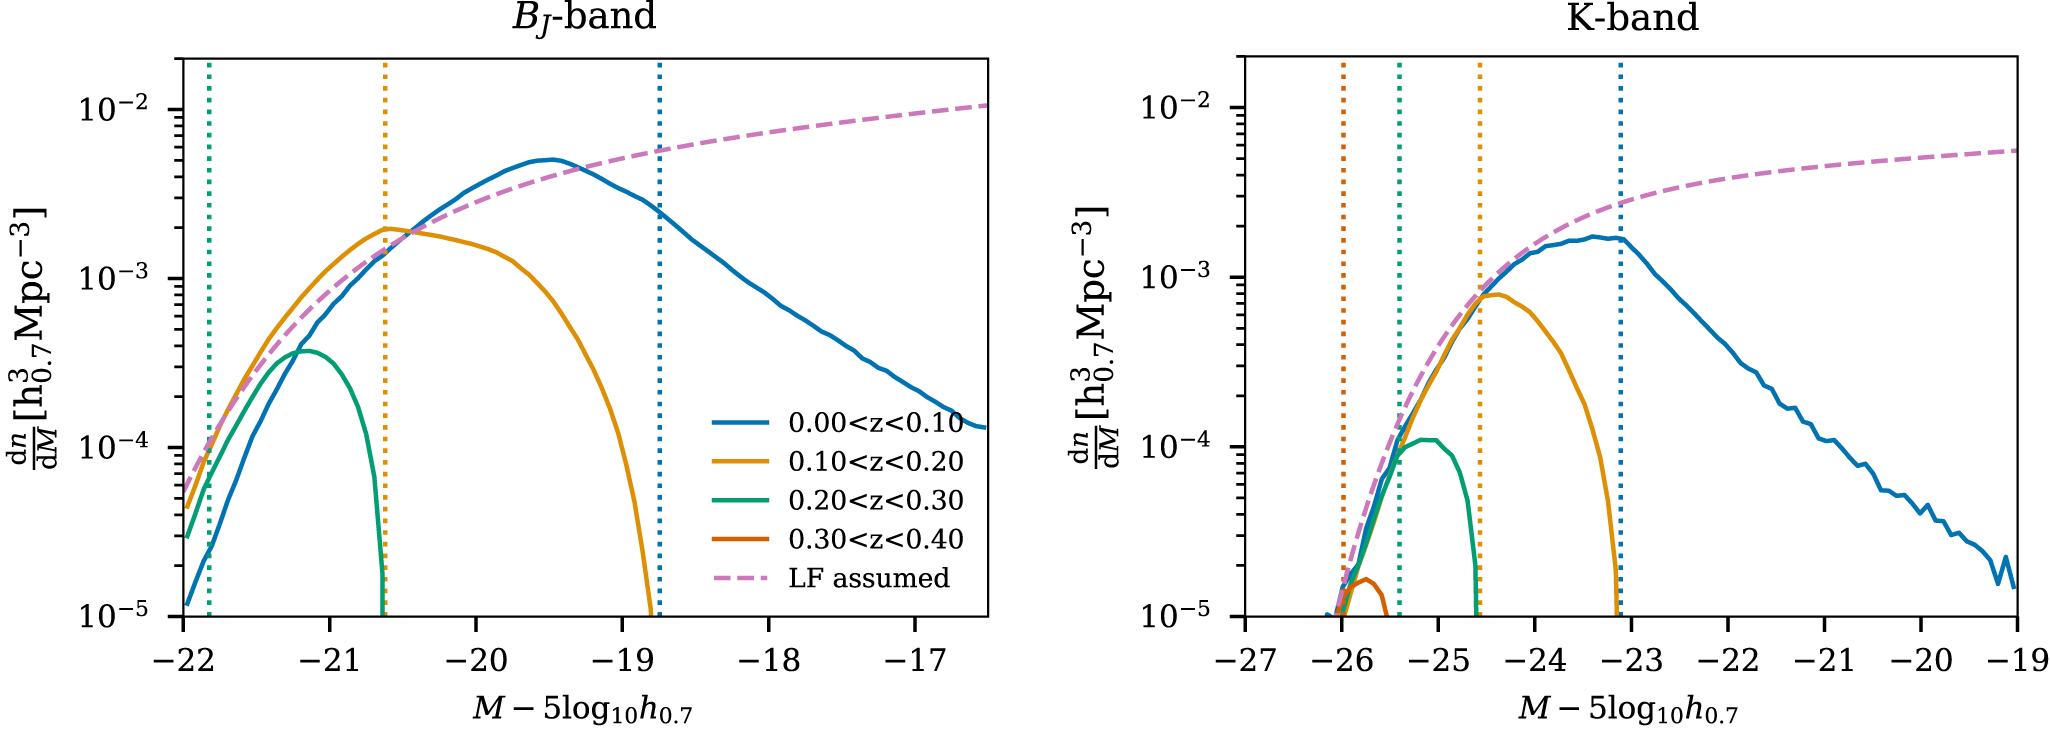
\includegraphics[width=\textwidth]{figures/apjac74bbf15_hr.jpg}
    \caption[The $B_J$-band and $K$-band luminosity function for the \texttt{GLADE+} catalog.]{The $B_J$-band (left) and $K$-band luminosity function (right) for the \texttt{GLADE+} catalog. The solid lines show the luminosity function of the catalog, while the dashed lines shows the assumed Schechter function. The vertical dashed line indicates the median absolute magnitude threshold for galaxy detection. The bright end of the $K$-band luminosity seems to match the assumed Schechter function, while the $B_J$-band luminosity function does not. This indicates that the assumption of a magnitude-limited catalog is not valid for the $B_J$-band~\citep{abbott2023constraints}.}
    \label{fig:luminosity_function}
\end{figure}

For modelling the out-of-catalog contribution, a Schechter luminosity function is assumed, which describes the distribution of galaxy luminosities in a given band. Wrong assumptions on the Schechter parameters, or incorrect description of selection biases can lead to biases in the inferred Hubble constant. The key assumption in constructing the out-of-catalog contribution is that the galaxy catalog is magnitude limited, i.e. galaxies are not detected only because they are too faint. If other selection biases (based on e.g., colors or spectral features) were present, the out-of-catalog contribution would be biased, leading to an incorrect estimate of the redshift prior \citep{abbott2023constraints}. 

If the assumption of a magnitude-limited catalog is valid, then the luminosity function of the galaxy catalog would match the assumed Schechter function at its bright end, and start to decrease as it reaches the corresponding absolute magnitude threshold. As can be seen in Figure~\ref{fig:luminosity_function}, this is indeed the case for the $K$-band luminosity function in \texttt{GLADE+}, which is well described by the assumed Schechter function. The $B_J$-band luminosity function, on the other hand, is not well described, and the assumption of a magnitude-limited catalog is not valid as there seem to be some additional missing galaxies at low redshift. This could lead to an incorrect estimate of the out-of-catalog contribution, and therefore an incorrect estimate of the redshift prior \citep{abbott2023constraints}. For this reason, traditionally, the $K$-band luminosity has been used for galaxy weighting in \ac{GW} cosmology inference pipelines. Another reason for using the $K$-band is, that the $K$-band luminosity is better correlated with the stellar mass of the galaxy, making it a more reliable tracer of the underlying matter distribution \citep{strazzullo2006near,sureshkumar2021galaxy,abbott2023constraints}. 

However, this choice is not without its limitations. The $K$-band luminosity is not always available for all galaxies in the catalog, leading to potential biases in the selection of galaxies used to construct the redshift prior. For example, the $K$-band luminosity is only available for about 1 million galaxies in the \texttt{GLADE+} catalog, which is a small fraction of the total number of galaxies in the catalog. This can lead to uncertainties in the redshift prior, which can in turn affect the inferred value of the Hubble constant. However, this effect should be relatively small, as we are interested in the overall matter distribution, and the $K$-band luminosity is a good tracer of the underlying matter distribution. This also forms the basis for this thesis, as we will be using the brightest galaxies in the $K$-band, in the \texttt{GLADE+} galaxy catalog, to trace the underlying matter distribution for improved $H_0$ inference as discussed in the next section.

\section{Refining the Redshift Prior: Brightest Galaxies as Tracers}
\begin{figure}[h!]
    \centering
    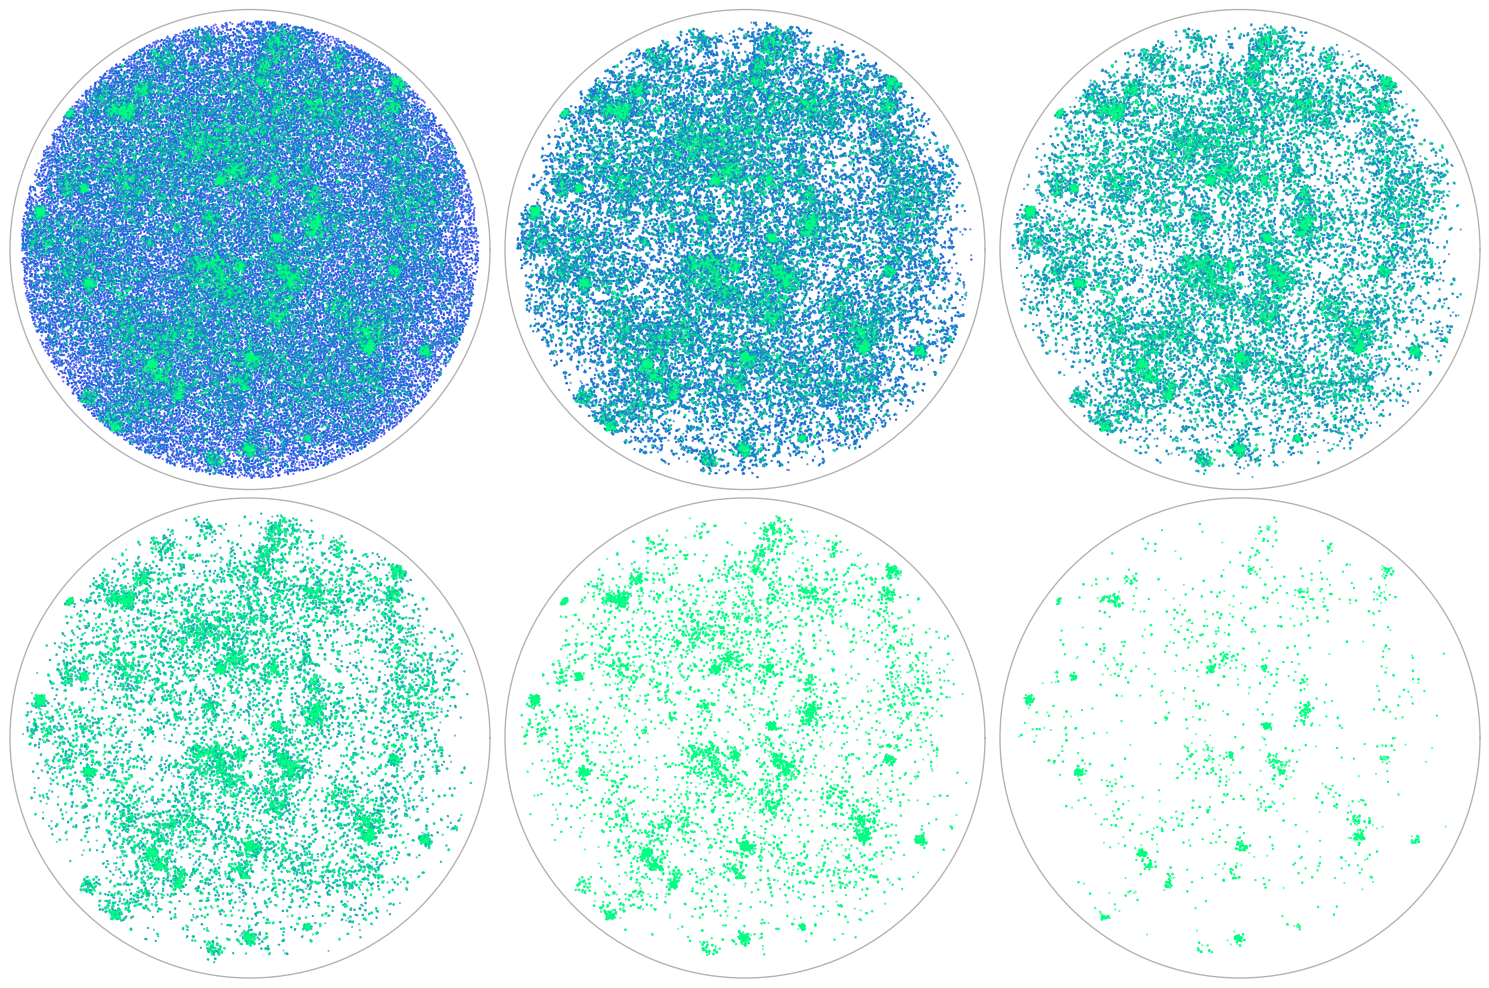
\includegraphics[width=\textwidth]{figures/depict7.png}
    \caption[Illustration of the proposed method, using bright galaxies as redshift tracers.]{Illustration of the proposed method for refining $H_0$ inference using the brightest galaxies as redshift tracers. The panels show different brightness cuts being applied to a galaxy catalog. The top left panel shows the case with a full galaxy catalog, while the subsequent panels (left-to-right) show the effect of applying increasingly strict brightness cuts. These depict how we can trace the matter distribution by using only the brightest galaxies. The last two panels (bottom center and right) show overly restrictive cuts, which would lead to a loss of information and a biased result. This is a conceptual visualization, generated with AI assistance, intended to represent the methodology rather than actual observational data.}
    \label{fig:depict}
\end{figure}

The current state of the art in dark siren cosmology relies heavily on the quality and completeness of the galaxy catalog used to construct the \ac{LOS} redshift prior. 
%The incompleteness of the galaxy catalog can lead to significant uncertainties in the redshift prior, which can in turn affect the inferred value of the Hubble constant. This is particularly important for dark sirens, as they rely on the statistical association of \ac{GW} events with galaxies in the catalog. 
The incompleteness of the galaxy catalog can lead to biases in the inferred redshift distribution, which can affect the accuracy of the Hubble constant measurement. State of the art dark siren methods have been developed to account for the incompleteness, but they still rely on the quality and completeness of the galaxy catalog used.

%While the statistical dark siren framework is powerful, its precision is ultimately limited by catalog incompleteness and the resulting need to model out-of-catalog galaxies. 
One strategy to mitigate this limitation is by refining the construction of the redshift prior by focusing on the \textit{brightest galaxies} to trace the underlying matter distribution. This would effectively make the catalog more complete and increase precision without introducing significant bias. The rationale is that the brightest galaxies are more likely to be associated with massive halos, which are in turn more likely to host detectable \ac{GW} events. The brightest galaxies are also more likely to be catalogued, as they are easier to detect and measure. These galaxies would also crudely trace the underlying matter distribution, since they are more likely to be associated with massive halos. This would be particulary useful for dark sirens, as they rely on the statistical association of \ac{GW} events with galaxies in the catalog. By replacing the redshift of the true host galaxy with the redshift of a nearby bright galaxy in the catalog, the small error incurred would be insignificant compared to the overall uncertainty in the redshift prior and the luminosity distance measurement.

Figure~\ref{fig:depict} illustrates this approach, highlighting how the brightest galaxies can be used to trace the underlying matter distribution. The last two panels in the figure show an overly restrictive cut, which would lead to a loss of information and a biased redshift prior. This emphasizes the importance of selecting an optimal brightness cut that balances the need for completeness with the desire for precision. The goal would be to find the optimal brightness cut that maximizes the precision of the redshift prior while minimizing bias.

This approach, of using the brightest galaxies to trace the matter distribution, is similar to the \textit{\ac{BCG}} method used in traditional cosmology, where the brightest galaxy in a cluster is used as a standard candle. The \ac{BCG} method has been shown to be effective in reducing the scatter in distance measurements and improving the precision of cosmological constraints \citep{lauer2014brightest}. By applying a similar approach to dark sirens, one can potentially improve the precision of the inferred Hubble constant without introducing significant bias.

To implement this approach, we define a subset of the \texttt{GLADE+} galaxy catalog, \texttt{GLADEPXX}, which includes only the top $XX\%$ of galaxies ranked by $K$-band luminosity, as the $K$-band luminosity is better associated with the mass of the galaxies \citep{strazzullo2006near,sureshkumar2021galaxy}. The construction of the LOS redshift prior is then modified to account for this restricted catalog. Specifically, the Schechter luminosity function is adjusted to reflect the brighter subset, making the out-of-catalog contribution smaller, effectively making the catalog more complete. This modified prior is then used in the Bayesian framework to infer the Hubble constant.

The next chapters provide a detailed description of the methodology, including the \texttt{gwcosmo} inference pipeline, the selection criteria for \texttt{GLADEPXX}, the modeling of the out-of-catalog part and the validation of this approach using mock data.